\chapter{Architettura dell'algoritmo di segmentazione}\lb{ALG}

In questo capitolo \e presentato l'algoritmo di segmentazione sviluppato che permette di
individuare la macchia attraverso una descrizione compatta del suo contorno, in vista delle
successive misure di dimensioni, forma, simmetrie, etc. 

%...........................................................................................
\subsubsection{La struttura dell'algoritmo}

L'algoritmo \e composto di due blocchi principali
\ben
{\it
\im condizionamento dell'immagine e inizializzazione del contorno attivo (snake);
\im evoluzione del contorno fino alla conclusione del processo di segmentazione.
}
\een

%===========================================================================================
\section{Algoritmo: Fase 1}

In questa prima fase l'immagine viene elaborata in modo da migliorare la qualit\a
della primitiva che si considera ai fini della segmentazione (nel nostro caso il colore) eliminando gli
elementi di disturbo che possono compromettere la localizzazione dei contorni che in questa applicazione
sono soprattutto i peli i quali possono intersecare la macchia o peggio essere vicini al
contorno tanto da coprirlo.
Rientra in questa fase anche il problema dell'inizializzazione del controrno attivo che
poi evolver\a fino a descrivere l'oggetto della segmentazione: la macchia cutanea.

%--------------------------------------------------------------------------------------------
\subsection{Condizionamento dell'immagine}

Nel Capitolo \r{OEDI} si sono introdotte alcune rappresentazioni dello spazio dei colori
che presentano delle propriet\a che le rendono preferibili al modello $RGB$ come
lo spazio $HSI$ (o $HSV$) e la {\it trasformata di Karhunen-Lo\`eve} (o di
{\it Hotelling}).
Vista la natura del problema, per cui si considera un solo elemento connesso e uniforme
(rispetto al colore) circondato da una zona anch'essa uniforme, sembrerebbe sufficiente
considerare la componente di $Hue$.
La sola tonalit\a per\o \e soddisfacente nel caso in cui si abbia una illuminazione sufficientemente
uniforme e non vi siano eccessivi effetti di riflessione.
Risultati migliori si ottengono invece elaborando le componenti della {\it trasformata di Karhunen-Lo\`eve} \cite{Lucchese} \cite{Schmid}.

%...........................................................................................
\subsubsection{Attenuazione degli elementi di disturbo}

Utilizzzando quest'ultima trasformata \e possibile predisporre una strategia per eliminare
alcuni disturbi presenti quali i peli, che generalmente appaiono come strutture con una
elevata correlazione lungo una direzione e il cui spessore non \e sempre trascurabile in 
relazione alle dimensioni della macchia.

Si pu\o utilizzare un filtro passa-basso, ad esempio gaussiano, o un
filtro a mediana che rispetto al precedente permette di ottenere un'immagine con una maggior
definizione dei contrasti.

Ma a causa delle dimensioni trasversali dei peli e del fatto che non \e nota la direzione lungo
la quale si sviluppano anche nel secondo caso \e necessario considerare per il filtro una
finestra $n \times n$ di pixels abbastanza grande ($n$ dell'ordine di $10 \div 15$) con
dei risultati comunque non soddisfacenti (Figura \r{elpeli}).

Altre soluzioni pi\u complesse considerano l'impiego degli operatori morfologici
\cite{Schmid} combinando opportunamente le operazioni di chiusura e apertura (vedi Capitolo
\r{OEDI}) con un'opportuna scelta del nucleo (o {\it structuring element}).

\begin{figure}[tbp]
 \centerline{
  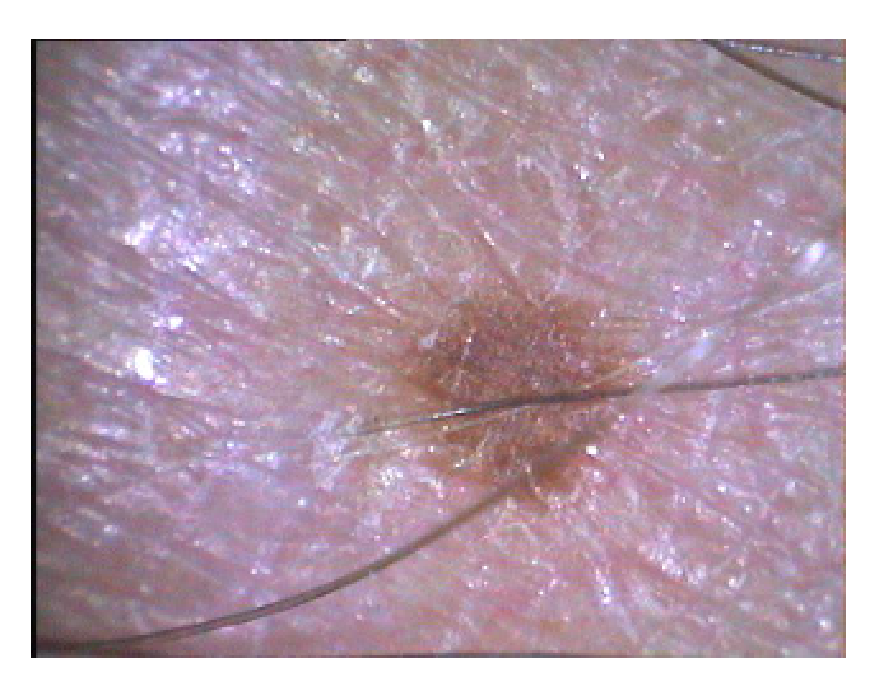
\psfig{file="./images/cpeli.eps",height=5cm,clip=}
  \hfill
  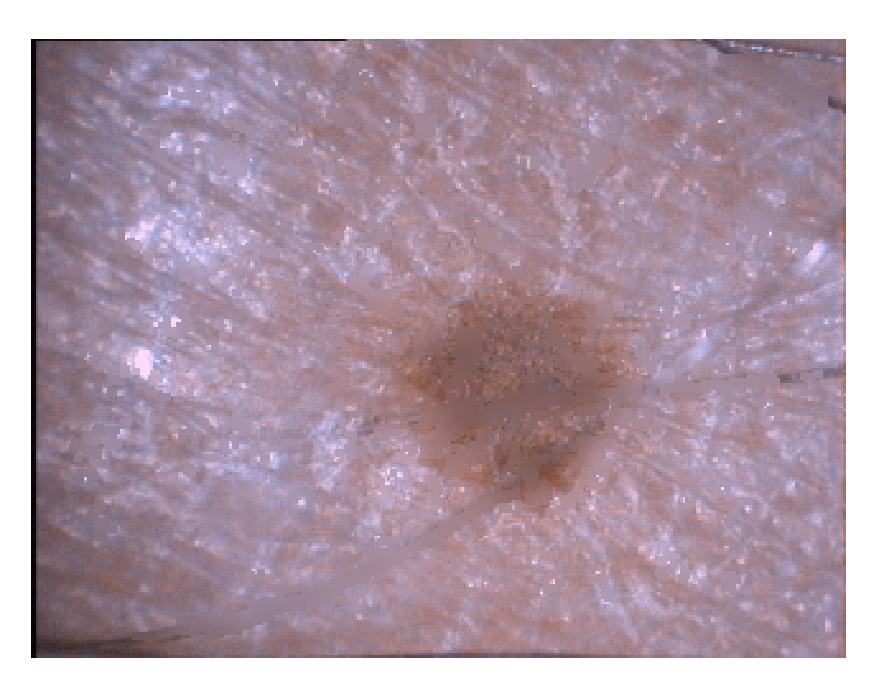
\psfig{file="./images/spelio.eps",height=5cm,clip=}}
 \centerline{
  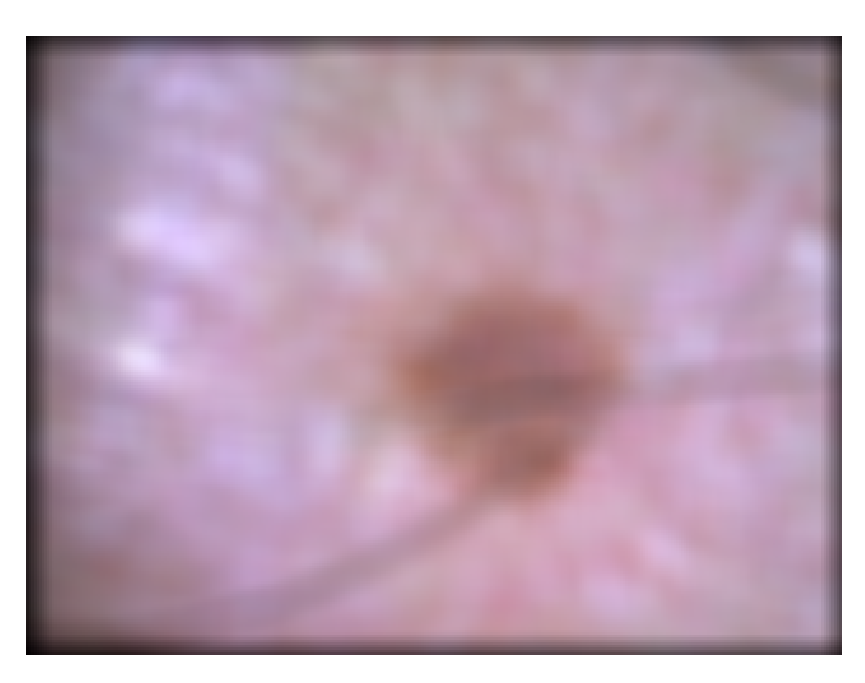
\psfig{file="./images/spelig.eps",height=5cm,clip=}
  \hfill
  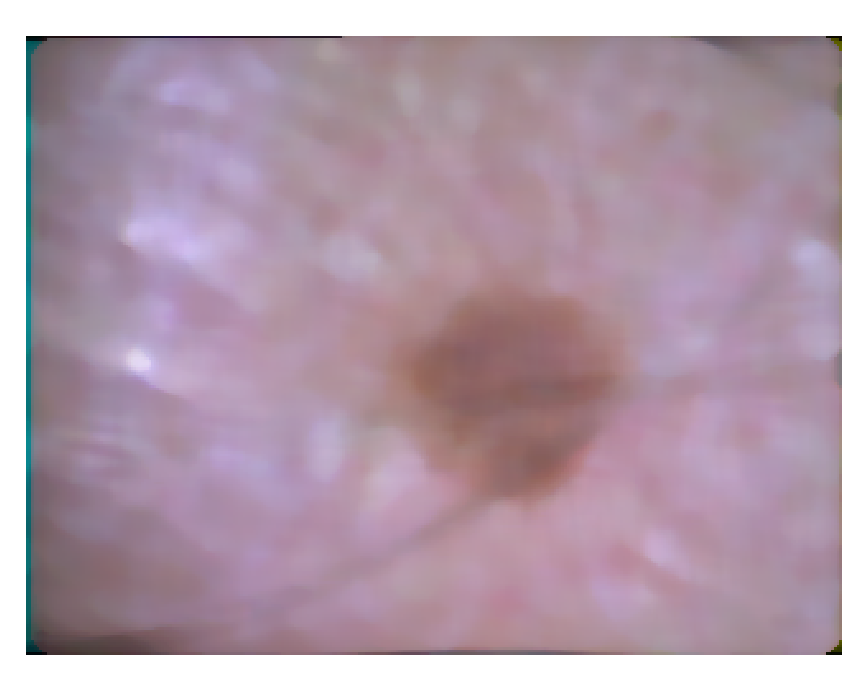
\psfig{file="./images/spelim.eps",height=5cm,clip=}}
 \caption[Attenuazione degli elementi di disturbo: peli]
  {Attenuazione degli elementi di disturbo: peli.\\
   {\sl In alto a sinistra \r{elpeli}.a}. Immagine originale.
   {\sl In alto a destra \r{elpeli}.b}. Utilizzo della
   misura di anisotropia definita dalla (\r{lam}) applicata alla componente principale della
   {\it trasformata di K.-L.} seguita da una sogliatura per individuare i punti pi\u probabilmente
   appartenenti ai peli. Quindi si \e sostituita una finestra circostante a ciascun punto con
   il valore di mediana della stessa.
   {\sl In basso a sinistra \r{elpeli}.c}. Applicazione del filtro passa-basso gaussiano.
   {\sl In basso a destra \r{elpeli}.d}. Applicazione filtro a mediana su tutta l'immagine.}
 \lb{elpeli}
\end{figure}

Si \e considerato invece di utilizzare un operatore locale, come
la stessa mediana, applicato per\o non su tutta l'immagine ma solo in corrispondenza del
disturbo individuato attraverso la misura di anisotropia definita dalla (\r{lam}).
La misura \e effettuata sulla prima componente della {\it trasformata di K.-L.} e la mappa che se
ne ottiene \e in scala di grigio con i valori massimi in corrispondenza
dei punti che appartengono a zone dell'immagine ad alta correlazione lungo una direzione.
Comunque fra i punti individuati non tutti appartengono ai peli, per cui \e necessario
introdurre un valore di soglia per selezionare quelli aventi una misura sufficientemente
elevata.

Ai punti individuati dalla sogliatura \e possibile quindi applicare un operatore locale, 
ad esempio un filtro a mediana come in Figura \r{elpeli}.

%--------------------------------------------------------------------------------------------
\subsection{Inizializzazione del contorno attivo - snake}

%.........................................................................................
\subsubsection{Motivazione}

Tenendo presente che l'immagine su cui si lavora non \e perfettamente binaria \e opportuno,
anche in relazione ai problemi di tempi di calcolo dell'evoluzione dello snake, definire
un contorno iniziale che sia il pi\u possibile prossimo a quello reale. 

Una possibilit\a \e quella di richiedere all'utente di definire alcuni punti e, ad esempio,
considerarli come i control points di una curva a B-splines e quindi costruire la curva 
che li approssima; oppure procedere ad una grossolana pre-segmentazione utilizzando
delle tecniche di binarizzazione.

Si considera in particolare quest'ultimo caso che comunque richiede un minimo apporto da parte
dell'utente che deve preselezionare sull'immagine originale un'opportuna finestra
che contenga il neo.

%.........................................................................................
\subsubsection{Processo di inizializzazione semiautomatica}

A partire dalla componente principale della {\it trasformata di K.-L.}, si effettua una riduzione 
della risoluzione applicando la (\r{campion}) ottenendo una consistente
diminuzione dei dati da analizzare e quindi del carico computazionale dei passi
successivi, sempre nell'ipotesi di approssimazione a cui si \e fatto riferimento.

Si procede quindi alla binarizzazione dell'immagine ottenuta con
i metodi indicati in (\r{segbin}).
\boss
Occorre tener presente che gli algoritmi indicati, per ragioni di efficienza, considerano
come oggetto di indagine l'istogramma del-l'immagine e non l'immagine completa,
per cui se l'area occupata dalla macchia \e circa uguale a quella circostante allora
l'istogramma normalizzato risulta abbastanza bimodale approssimando il meglio
possibile le ipotesi di validit\a su cui si basano gli algoritmi di binarizzazione.
Tale condizione pu\o essere condizionata dalla scelta dell'area da analizzare fatta
dall'utente.
\eoss

Per quanto riguarda i due metodi presentati si \e preferito quello iterativo in quanto,
fissata la tolleranza sull'approssimazione del valore di soglia in modo che non sia
eccessivamente restrittiva, si ottengono gli stessi risultati del caso dell'algoritmo di
classificazione ma in tempi inferiori.



Il risultato \e del tipo di Figura \r{neobin} in cui si pu\o notare come
non vi sia un unico elemento connesso e con contorni ben definiti, per cui si procede 
applicando in due passi successivi due operatori morfologici per ottenere una sola regione
compatta:
\ben
\im con una prima operazione di {\it apertura} si eliminano piccoli disturbi isolati e 
    l'eccessiva frastagliatura del contorno dell'elemento principale (Figura \r{neomorf}.a);
\im successivamente con un'operazione di {\it chiusura} si ottiene un unico elemento 
    compatto e, adottando un nucleo (o {\it structuring element}) circolare, con i bordi "regolari
    ({\it smooth})" (Figura \r{neomorf}.b).
\een

\begin{figure}[tbp]
 \centerline{
  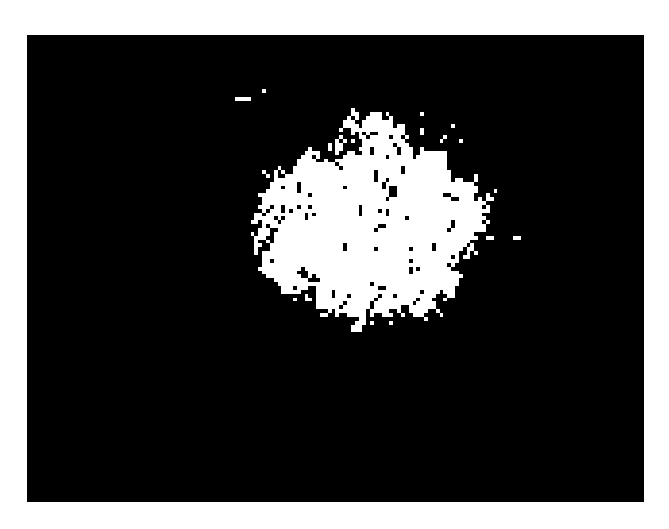
\psfig{file="./images/neobin2.eps",height=6cm,clip=}}
 \caption[Esempio di binarizzazione]
  {Esempio di binarizzazione ottenuta determinando il valore di soglia con il metodo
   iterativo proposto in (\r{segbin}). L'istogramma \e definito rispetto una regione
   definita dall'utente che circonda la macchia in modo che l'area occupata da quest'ultima
   sia prossima a quella complementare. (l'immagine riportata
   \e invece completa e non solo limitata alla finestra selezionata).}
 \lb{neobin}
 \centerline{
  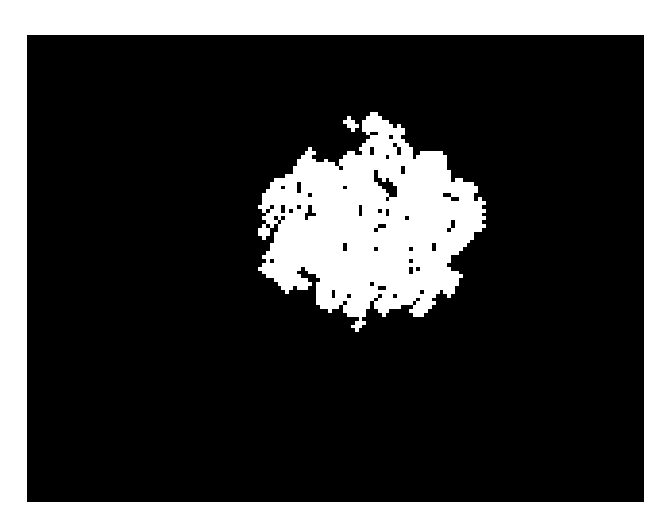
\psfig{file="./images/neobo2.eps",height=5cm,clip=}
   \hfill
  
\psfig{file="./images/neoboc2.eps",height=5cm,clip=}}
   \caption[Esempio di applicazione di operatori morfologici]
    {{\sl A sinistra \r{neomorf}.a}. Applicazione dell'operatore di apertura all'immagine binaria di
     Figura \r{neobin}: permette di eliminare i piccoli disturbi isolati e l'eccessiva 
     frastagliatura del contorno.
     {\sl A destra \r{neomorf}.b}. Applicazione dell'operatore di chiusura all'immagine di sinistra con lo
     scopo di ottenere un unico elemento compatto e con i bordi regolari; si \e perci\o
     utilizzato un nucleo (o {\it structuring element}) circolare.}
 \lb{neomorf}
\end{figure}

Il contorno attivo o {\it snake} iniziale \e ottenuto a partire dal bordo della regione appena
individuata ricorrendo ancora ad opportuni operatori morfologici:
\bdf
Sia B l'immagine binaria e K lo {\it stucturing element} scelto fra i due seguenti
$$
K\,=\,\qmatrix{1 & 1 & 1 \cr
               1 & 1 & 1 \cr
               1 & 1 & 1 \cr} \qquad o \qquad
K\,=\,\qmatrix{0 & 1 & 0 \cr
               1 & 1 & 1 \cr
               0 & 1 & 0 \cr}
$$
noti come $8-neighborhood$ e $4-neighborhood$ rispettivamente; allora l'insie-me dei punti
o pixel della matrice B che definiscono il contorno $\Gamma$ \e definito
$$
\Gamma\,=\,B\,/\,(B \ominus K)\,=\,B\,\cap\,\overline{(B \ominus K)}\,=\,
B\,\cap\,(\overline{B} \oplus K)
$$
\edf

Una volta individuato il contorno si determina la curva a {\it B-spline cubiche uniformi} che
la approssima.
Di seguito sono indicati i passi del procedimento:
\ben
\im l'insieme $\Gamma$ \e definito dai pixel $p(r,c)$, $r \in \{1,\dots,R\}$ e $c \in \{1,\dots,C\}$,
    le cui coordinate sono espresse in termini di coppie riga-colonna; per cui le si trasforma
    nel sistema di riferimento cartesiano $X-Y$;
\im i punti, nel nuovo sistema di riferiemnto, vengono ordinati in senso antiorario   
     \footnote{Oppure si parte da una descrizione del contorno in pixel gi\a definita
              in senso antiorario utilizzando ad esempio una rappresentazione tipo
              {\it chain code}.
     		  
     		  Il senso antiorario \e considerato il verso di percorrenza positivo della curva;
              risulta determinante nella relazione fra il versore tangente alla curva
              e la normale esterna.}; 
\im definendo un opportuno criterio di complessit\a \e possibile stabilire il numero di
    {\it spans} e quindi di {\it control points} (si veda il Capitolo \r{BSC}) 
    con cui descrivere una curva a B-splines che approssimi la curva di cui tali punti
    si considerano dei campioni. Per determinare i {\it control points} si procede alla
    soluzione di un sistema di equazioni lineari caratterizzato da un numero di incognite
    (i {\it control points}) inferiore ai valori noti (i punti campioni della curva)
    risolvendo un problema ai minimi quadrati;
\im considerando che la curva \e ottenuta dall'immagine originale ad una risoluzione ridotta
    occorre effettuare un cambiamento di scala opposto per riportarla
    nell'immagine originale tenendo presente che va aggiornata la componente di traslazione
    della trasformazione che lega i due sistemi di riferimento adottati: quello immagine
    e quello della curva.
\een

La definizione del criterio di complessit\a e il problema della determinazione dei 
{\it control points} sar\a esposto nei paragrafi successivi.

%===========================================================================================
\section{Algoritmo: Fase 2}

La seconda fase \e caratterizzata dall'evoluzione del contorno definito nella fase
precedente fino a raggiungere una condizione di equilibrio. Si considera come modello dello
snake la curva a B-splines cubiche uniformi la cui legge di evoluzione nel tempo \e definita
dall'algoritmo di {\it Yezzi, Tsai e Willsky} trattato in (\r{AYTW}).
\`E proposto inoltre un criterio per misurare la complessit\a del contorno della regione
da segmentare per ridefinire il numero e la distribuzione dei {\it control points}.

\balg
{\bf Evoluzione dello snake.}\par
\ben
\im \lb{PAYezzi1} A partire dal vettore dei control points ${\bf Q}$ e fissato il numero di campioni $N(i)$
    per lo span $i-esimo$, con $i=1,\dots,N_s$ con $N_s$ numero di spans della curva chiusa
    pari al numero di punti di controlllo, si pu\o calcolare il vettore ${\bf X}$ dei 
    campioni della curva. 
    Successivamente si calcolano i versori tangenti ${\bf X}_s$ e normali ${\bf X}_n$ alla
    curva nei punti ${\bf X}$ e la curvatura $k$ della curva in ${\bf X}$.
\im Calcolo di aree e medie interne ed esterne e dalla (\r{EYezzi}) lo stato energetico
    dello snake.
\im Se si \e raggiunta la condizione di minima energia, rispetto alle condizioni fissate,
    allora il processo di segmentazione \e concluso, altrimenti si continua con
    l'aggiornamento della curva.
\im Con il passo di aggiornamento si determina il nuovo vettore di punti ${\bf Y}$
    ottenuto da ${\bf X}$ secondo la legge di evoluzione definita dalla discretizzazione della
    (\r{flow}).
\im Ogni $T$ passi \e possibile aumentare il numero dei punti di controllo $N_s$ e 
    ridistribuire i campioni ${\bf Y}$ della curva secondo il criterio di complessit\a fissato. 
\im A partire da ${\bf Y}$ e $N_s$ (o eventualmente i loro aggiornamenti) si determina il nuovo
    vettore ${\bf Q}$ dei punti di controllo che definisce la curva a B-splines che meglio
    approssima, ai minimi quadrati, la curva i cui campioni sono dati da ${\bf Y}$.
\im Si ritorna al passo \r{PAYezzi1}.
\een
\ealg

Vediamo ora in dettaglio i singoli passi.

%--------------------------------------------------------------------------------------------
\subsection{Passo 1: calcolo di ${\bf X}$, ${\bf X}_s$, ${\bf X}_n$, $k$}

\`E possibile esprimere tali vettori in funzione dei punti di controllo definendo opportune
matrici ${\bf A}$, ${\bf A}_s$ e ${\bf A}_{ss}$ (si veda l'Appendice \r{A2}).\par
Considerata la curva chiusa $\Gamma$ descritta per mezzo delle B-splines cubiche e 
uniformi dalla carta ${\bf r}(s,t)$ e discretizzandola rispetto alla variabile $s$ \e possibile
ottenere il vettore dei campioni
\be
{\bf X}\,=\,{\bf A}\,{\bf Q}
\ee
I versori ${\bf \tau}$ tangenti alla curva sono definiti, nel continuo, dalla
\be
{\bf \tau}({\bf r}(s,t))\,=\,\frac{{\bf r}_s(s,t)}{\|{\bf r}_s(s,t)\|}
\ee
che applicata ai punti di ${\bf X}(i)$, $i=1,\dots,N_p$ risulta
\be
{\bf \tau}({\bf X}(i))\,=\,\frac{{\bf X}_s(i)}{\|{\bf X}_s(i)\|} \quad con \quad {\bf X}_s\,=\,{\bf A}_s\,{\bf Q}.
\ee
Considerato che ${\bf \tau}$ definisce l'orientamento positivo di percorrenza della curva,
che qui \e considerato antiorario, \e possibile calcolare la normale esterna ${\bf n}$ non
appena si fissi l'orientamento positivo del piano che \e considerato dal versore ${\bf e}_3$;
per cui risulta
\be
{\bf n}({\bf r}(s,t))\,=\,{\bf \tau}\wedge{\bf e}_3({\bf r})\,=\,(\tau_y,-\tau_x,0)
\ee
e che si riduce alla coppia $(\tau_y,-\tau_x)$; quindi esprimibile dalla 
\be
{\bf n}({\bf r}(s,t))\,=\,\smatrix{2}{ 0 & 1 \cr
                                      -1 & 0 \cr}{\bf \tau}
\ee
Riferito ai campioni della curva vale
\be
{\bf X}_n(i)\,=\,\smatrix{2}{ 0 & 1 \cr
                       -1 & 0 \cr}{\bf \tau}(X(i)).
\ee

Per quanto riguarda la curvatura si considera la definizione
\be
k({\bf r}(s,t))\,=\,\frac{{\bf r}_s(s,t) \wedge {\bf r}_{ss}(s,t)}{\|{\bf r}_s(s,t)\|^3}
\ee
che rappresenta la curvatura con segno della curva ${\bf r}(s,t)$; che si semplifica nella
\be
k({\bf X}(i))\,=\,\frac{{\bf X}_s(i) \wedge {\bf X}_{ss}(i)}{\|{\bf X}_s(i)\|^3}
\ee
dove ${\bf X}_{ss}={\bf A}_{ss}\,{\bf Q}$.
\`E possibile definire anche il vettore curvatura diretto lungo la normale esterna
${\bf k}\,=\,k\,{\bf n}$.

%--------------------------------------------------------------------------------------------
\subsection{Passo 2: calcolo delle medie e aree interne ed esterne alla curva}

La funzione energia definita da Yezzi et al. \cite{Yezzi} e la relativa legge di aggiornamento
prevedono il calcolo del vettore delle medie e delle aree delle regioni interna ed esterna
rispetto alla curva chiusa.

Considerando che dalla Fase 1 si ottiene una curva iniziale che \e abbastanza
prossima al contorno finale \e conveniente applicare la versione locale suggerita nello stesso
articolo: ovvero la regione interna compresa fra la curva $\Gamma$ e la curva interna
$\Gamma^{int}$ e la regione esterna fra $\Gamma$ e $\Gamma^{est}$.

Le due nuove curve possono essere ottenute sfruttando quanto visto a proposito dell'invarianza
delle curve a B-splines nei confronti delle omotetie (Figura \r{omotetia}).

Sfruttando la versione locale si evita di dover considerare la zona vicine
ai bordi dell'immagine maggiormente soggetta ai disturbi dovuti agli effetti di bordo
dell'ottica del sensore e ad una illuminazione non uniforme.

%--------------------------------------------------------------------------------------------
\subsection{Passo 3: la condizione di equilibrio}

L'evoluzione dello snake termina quando la funzione energia ha raggiunto il punto di minimo
ovvero, come punto di estremo, ha gradiente nullo.
Fra le due condizioni, teoricamente equivalenti, si \e scelta la prima in quanto pi\u
semplice da determinare una volta note le due medie; la seconda infatti richiede di 
verificare che l'incremento fra due istanti successivi \e trascurabile per ogni campione della
curva.

In condizioni ideali la funzione ${\cal E}(t)$, che descrive l'andamento dell'energia durante
l'evoluzione dello snake, \e monotona decrescente fino alla condizione di equilibrio, e
poi rimane costante, per cui il minimo \e individuato nel momento in cui vale
${\cal E}(t^\ast)={\cal E}(t^\ast +1)$ per i due istanti successivi $t^\ast$ e $t^\ast +1$.

Nelle condizioni reali invece ci\o non vale a causa delle approssimazioni introdotte e quindi
per stabilire il raggiungimento della condizione di equilibrio \e pi\u opportuno valutare
l'andamento dell'energia negli ultimi $T_e$ passi di calcolo; in particolare si considera
la funzione
\be
\epsilon(t)\,=\,\frac{1}{|{\cal E}(t)|}\,
                \frac{1}{T_e}\,\sum_{t-T_e+1}^{t}\,|{\cal E}(t)-{\cal E}(t-1)|
\ee

che rappresenta la media dei valori assoluti delle variazioni dell'energia totale degli
ultimi $T_e$ passi di calcolo relativa all'energia all'istante $t$.

Si considera ${\cal E}(t)$ "costante" quando $\epsilon(t)$ \e inferiore ad un valore
prefissato che essendo espresso in termini relativi \e indipendente dal valore di
${\cal E}(t)$.

%--------------------------------------------------------------------------------------------
\subsection{Passo 4: aggiornamento della curva in base alla legge di evoluzione}

Come detto si considera il modello di {\it snake} la cui legge di evoluzione \e data dalla (\r{flow})
\be
\frac{d \Gamma}{dt}\,=\,\sum_{j=1}^{N}\,(m_j^{int}-m_j^{est})\,
              \bigg[\frac{P_j-m_j^{int}}{A^{int}}\,+\,\frac{P_j-m_j^{est}}{A^{est}}\bigg].
\ee
Per poterla applicare \e necessario discretizzarla sia nella variabile spaziale sia in 
quella temporale; per quanto riguarda la prima si procede come sopra considerando i campioni
della curva dati da ${\bf r}_i$, mentre per la variabile temporale si approssima la
derivata con il rapporto incrementale (un'approssimazione del primo ordine):
\be
\frac{d \Gamma}{dt}\,=\,\frac{\Gamma (t + \Delta t)-\Gamma (t)}{\Delta t}
\ee
da cui si ottiene 
\be
\Gamma (t + \Delta t)\,=\,\Gamma (t)\,+\,\frac{d \Gamma}{dt}\,\Delta t
\ee
ovvero
\be
{\bf Y}(i)\,=\,{\bf X}(i,t + 1)\,=\,{\bf X}(i,t)\,+\,g(k_i)\frac{d \Gamma}{dt}\,({\bf X}(i))
\ee

\boss
Le coordinate dei campioni ${\bf X}$ sono definite in $[0,C]\times[0,R]\subset\M(R)^2$, mentre
le primitive $P_j$ sono definite per i pixels di coordinate $(r,c)$ appartenenti a
$\{1,R\}\times\{1,C\}\subset\M(N)^2$, con $R$ e $C$ numero di righe e di colonne, quindi \e
necessario poter stabilire l'intensit\a della primitiva da associare al campione della
curva.
Il punto $X(i)=(x_i,y_i)$ pu\o essere associato al pixel di riga $r=\lceil y_i \rceil$
e colonna $c=\lceil x_i \rceil$( \footnotemark ), per cui l'intensit\a della primitiva \e
$P(r,c)$.
\footnotetext{Si fa riferimento al caso in cui il sistema di riferimento cartesiano della
curva ha l'origine coincidente con lo spigolo in alto a sinistra della matrice $P$ e con
gli assi $X$ e $Y$ diretti lungo le colonne e le righe rispettivamente.}

Per tener conto che il punto non \e necessariamente al centro del pixel e del fatto che il
valore del pixel stesso potrebbe essere affetto da rumore \e opportuno considerare $P$ su una
finestra di pixel nell'intorno di quello fissato; ad esempio considerando la media pesata
o la mediana dei valori dei pixel della finestra.
\eoss

%.......................................................................................
\subsubsection{La funzione guadagno g(k)}

Si noti che l'"incremento temporale" $\Delta t$ \e stato conglobato nella
funzione $g(k)$ che definisce un opportuno guadagno che dipende dalla curvatura nel
punto $i-esimo$ $X(i)$.
La dipendenza del guadagno dalla curvatura permette di modulare l'incremento in funzione 
delle caratteristiche locali della curva riducendo il peso delle misure effettuate in
tratti ad elevata curvatura che potrebbero determinare la formazione di cappi.

Tenendo presente che $k$ \e la curvatura con segno, la funzione guadagno deve essere pari,
per cui una possibile scelta \e data dalla gaussiana
\be
g(k)\,=\,g_0\,\exp(- \alpha k^2)
\ee
dove $g_0$ \e il guadagno massimo e il fattore $\alpha$ definisce la forma del filtro.

La scelta di $g_0$ va fatta tenendo conto che se da un lato pu\o aumentare la velocità
dello {\it snake}, ovvero ridurre i tempi di convergenza, dall'altro pu\o renderlo instabile
o fare in modo che l'evoluzione si arresti su minimi relativi non corrispondenti al bordo
dell'oggetto che si vorrebbe identificare. 

%.......................................................................................
\subsubsection{Gli insiemi di livello}

Nell'articolo \cite{Yezzi} gli autori utilizzano gli {\it insiemi di livello} ({\it level set}) \cite{Malladi}
come soluzione per l'implementazione della legge di evoluzione; tale metodo permette inoltre
di realizzare in modo efficiente e automatico le operazioni topologiche di divisione e fusione
di {\it snakes} per poter individuare pi\u oggetti presenti nell'immagine a partire da una sola
curva oppure da pi\u curve ({\it semi}) disseminate sull'immagine.

La possibilit\a di realizzare tali trasformazioni non \e 
presente negli altri modelli di snake se non con l'aggiunta di procedure supplementari 
(come nel caso proposto in \cite{Terzopoulos}). 

Nel nostro caso comunque si \e scelto di adottare la legge espressa nella sua forma originale
e procedere a semplici discretizzazioni.

%--------------------------------------------------------------------------------------------
\subsection{Passo 5: il criterio di complessit\a della curva}

Nella fase di inizializzazione dello {\it snake} vengono individuati un certo numero di control
points che si ritiene sufficiente a descrivere il contorno dell'oggetto individuato dalla
binarizzazione, numero che potrebbe non essere comunque sufficiente in relazione alla
complessit\a effettiva dell'elemento da segmentare.

Durante l'evoluzione inoltre si pu\o trovare che un certo numero di campioni \e maggiormente
concentrato in un tratto della curva non eccessivamente complesso, e con essi anche un
maggior numero di control points, con conseguenze negative per la regolarit\a della curva
stessa (si veda \r{PSCBS}).
Si \e deciso perci\o di ricostruire una nuova sequenza di campioni da ridistribuire ad un
nuovo insieme di punti di controllo di dimensioni diverse dal precedente; in questo modo
si scorrela l'evoluzione della curva dai passi precedenti accelerando la convergenza al
risultato finale.

%.......................................................................................
\subsubsection{Ricampionamento della curva}

Dato il vettore di punti ${\bf Y}$ ottenuto nel passo precedente, si considera la poligonale
i cui vertici sono proprio gli elementi di ${\bf Y}$ e a questa si sovrappone un particolare
reticolo e si determinano le intersezioni ${\bf \Upsilon}(i)$ fra la poligonale e il reticolo:
quest'ultime costituiscono i nuovi campioni della curva (Figura \r{reticolo}).

\begin{figure}[tbp]
 \centerline{
  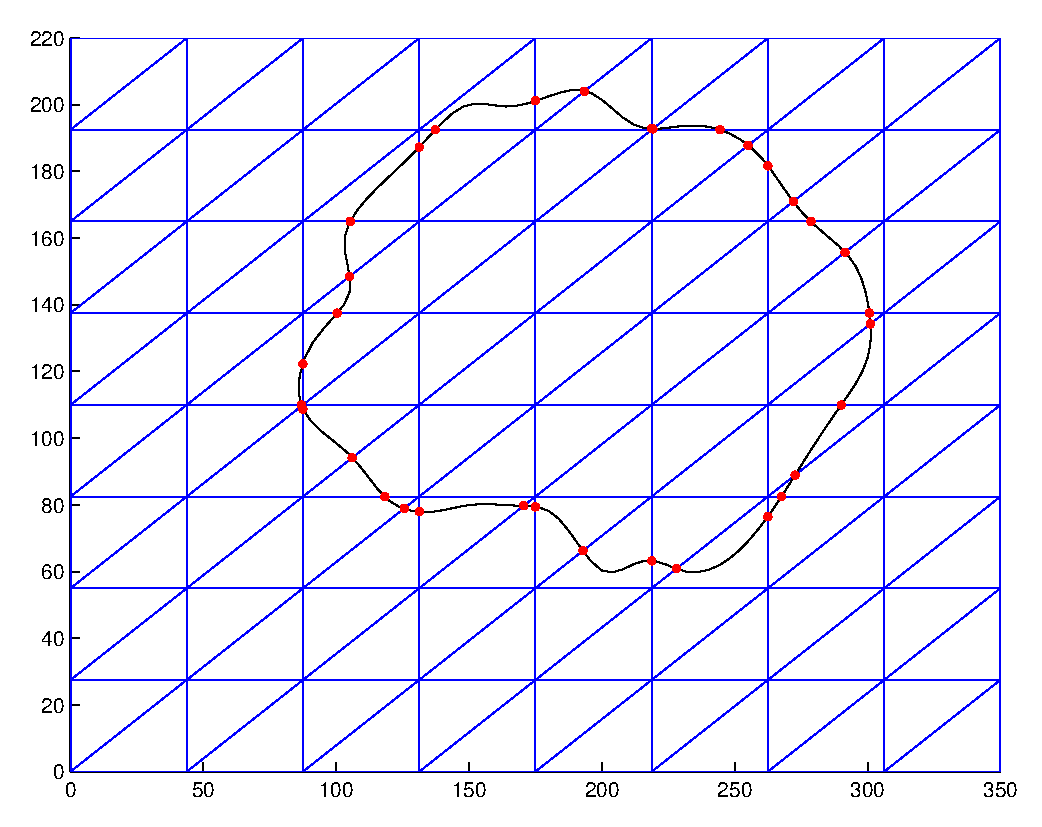
\psfig{file="./images/reticolo.eps",height=6cm,clip=}}
 \caption[Riparametrizzazione dello snake a B-splines]
  {Ricampionamento dello {\it snake} a B-splines realizzato intersecando la curva con un 
   reticolo ottenuto come scomposizione simpliciale, a simplessi triangolari, del piano
   immagine. I nuovi campioni ${\bf \Upsilon}(i)$ corrispondono alle intersezioni.}
 \lb{reticolo}
\end{figure}

Il reticolo introdotto rappresenta un esempio di {\it reticolazione simpliciale} o 
{\it triangolazione} del piano che risulta scomposto nella somma di {\it simplessi} topologici,
che nel caso in esame sono i singoli triangoli \footnotemark, che offre i seguenti vantaggi:

\footnotetext{La scomposizione simpliciale \e sviluppata nell'ambito della Topologia
Algebrica.}

\bi 
\im una rappresentazione univoca della curva;
\im variando la densit\a del reticolo \e possibile controllare il grado di 
approssimazione del contorno e di conseguenza anche
la velocit\a di convergenza al risultato finale.
\ei

Si osserva che la scelta della riparametrizzazione con l'uso della triangolazione simpliciale
\e utilizzata in \cite{Terzopoulos} per implementare le trasformazioni topologiche.
 
%.......................................................................................
\subsubsection{Definizione del criterio di complessit\a}

I nuovi campioni vengono successivamente distribuiti ai nuovi spans in modo che la 
complessit\a di ciascun span sia entro un limite massimo prefissato ${\cal M}$ interpretabile
come la "massa" totale dello span.

\bdf
{\bf Complessit\a.}\par
Per ciascun punto ${\bf \Upsilon}(i)$ si considerano i due vettori ${\bf u}(i)$ e ${\bf v}(i)$
$$
{\bf u}(i)=\frac{{\bf \Upsilon}(i-1)-{\bf \Upsilon}(i)}{L} \qquad
{\bf v}(i)=\frac{{\bf \Upsilon}(i+1)-{\bf \Upsilon}(i)}{L},
$$
normalizzati rispetto la lunghezza $L$ della poligonale di vertici ${\bf \Upsilon}(i)$, e le due
funzioni 
$$
d(i)\,=\,d({\bf u}(i),{\bf v}(i))\,=\,\|{\bf u}(i)\|+\|{\bf v}(i)\|
$$
$$
c(i)\,=\,c({\bf u}(i),{\bf v}(i))\,=\,\|{\bf u}(i)+{\bf v}(i)\|
$$
che descrivono i due contributi della complessit\a della "curva" nel punto: il primo tiene
conto della distanza fra i due vertici precedente e successivo, in senso antiorario, mentre
il secondo del grado di allineamento fra i tre punti (una sorta di curvatura).
Entrambi sono normalizzati rispetto alla lunghezza (perimetro) della poligonale in modo
da rendere il procedimento indipendente dalle dimensioni.

La complessit\a totale \e definita dalla combinazione dei due termini secondo i pesi $w_d$ e
$w_c$:
\be
\mu(i)\,=\,w_d\,d(i)\,+\,w_c\,c(i)
\ee
\edf

\boss
Nell'applicazione considerata, si sono ottenuti migliori risultati con $w_d > w_c$.
\eoss

Quindi nota la "densit\a" $\mu(i)$ si suddivide il vettore $\Upsilon$ in {\it spans} aventi
"massa" minore o al pi\u uguale a ${\cal M}$; in tal modo si determina la nuova
lunghezza del vettore dei control points $N_s^{\,\prime}$ per i quali vanno aggiornate le
matrici ${\bf A}$, ${\bf A}_s$ e ${\bf A}_{ss}$ che saranno utilizzate all'inizio del successivo
passo di evoluzione dello snake.

\begin{figure}[tbp]
 \centerline{
  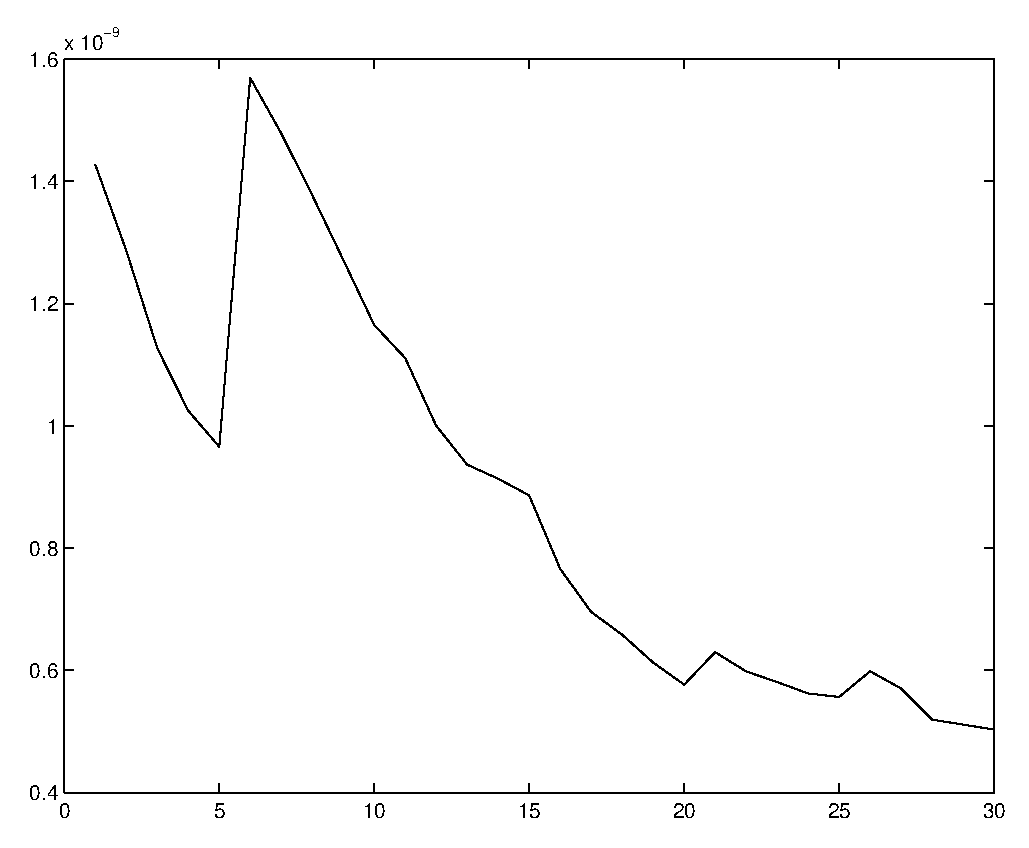
\psfig{file="./images/Ec.eps",height=5cm,clip=}
   \hfill
  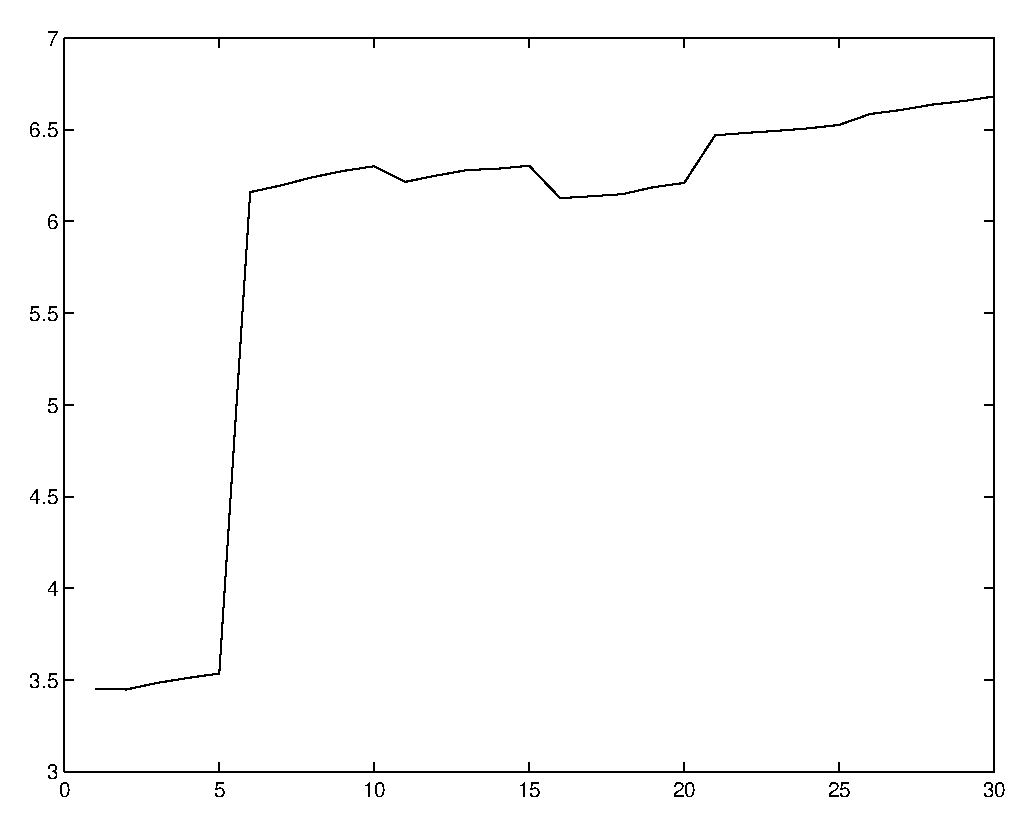
\psfig{file="./images/Et.eps",height=5cm,clip=}}
   \caption[Energie dello snake]
    {{\sl A sinistra \r{energie}.a}. Energia delle "forze" deformanti (si veda il testo).
     {\sl A destra \r{energie}.b}. Modulo dell'energia totale dello snake (\r{EYezzi}).}
 \lb{energie}
\end{figure}

In Figura \r{energie}.a mostra è rappresentato l'andamento dell'energia dei
campioni della funzione $(d \Gamma / dt)({\bf X}(i))$, ovvero la norma $L_2$ dello stesso vettore,
che si pu\o pensare indicativa delle "forze" deformanti che agiscono sullo {\it snake};
la \r{energie}.b mostra invece il modulo dell'energia dello snake valutata secondo la
(\r{EYezzi}).

Man mano che si procede verso lo stato di equilibrio finale si ha mediamente una diminuzione
della prima in quanto si \e sempre pi\u vicini all'o-biettivo finale (come se agisse una forza
elastica) mentre la seconda aumenta, ovvero l'energia con segno del sistema diminuisce,
coerentemente con le ipotesi fatte sullo stato di equilibrio a minima energia potenziale.

%--------------------------------------------------------------------------------------------
\subsection{Passo 6: la rappresentazione a B-splines della curva aggiornata}

Ad ogni ciclo sia che si abbia una ridistribuzione dei punti ${\bf \Upsilon}$ sia che si
considerino direttamente i punti ottenuti dal processo di aggiornamento $\bf Y$, si procede
alla determinazione della rappresentazione della curva a {\it B-splines 
cubiche uniformi} che approssima i campioni ottenuti calcolando il nuovo vettore di control points $\hat{\bf Q}$.

A partire dall'espressione definita precedentemente ${\bf X}={\bf A}\,{\bf Q}$, che lega i
control points ai campioni della curva, \e possibile ricavare una soluzione al problema
inverso ovvero ottenere i control points dai campioni ${\bf \Upsilon}$.

Per il sistema di equazioni lineari
\be
{\bf A}\,{\bf Q}\,=\,{\bf \Upsilon},
\ee
dove il numero di vincoli (equazioni) \e superiore al numero di incognite (${\bf Q}$), 
si considera il problema in termini di approssimazione ai minimi quadrati,
ovvero si considera come soluzione il vettore $\hat{\bf Q}$ per cui \e minima la norma 
$\|\,{\bf \Upsilon}\,-\,{\bf A}\,\hat{\bf Q}\|$.

La soluzione \e unica ed \e data da
\be
\hat{\bf Q}\,=\,{\bf A}^{\dagger}\,{\bf \Upsilon} 
\ee
dove ${\bf A}^{\dagger}=({\bf A}^{T}{\bf A})^{-1}){\bf A}^{T}$ \e la
{\it pseudo-inversa sinistra} di ${\bf A}$.
 
%===========================================================================================
\section{Risultati}

Nelle Figure \r{risIm}, \r{risIsa} e \r{risIp} sono visualizzati alcuni esempi di risultati
dell'ap-plicazione dell'algoritmo di segmentazione sviluppato.

Dalle Figure \r{risIm} e \r{risIsa} si pu\o notare che l'algoritmo \e abbastanza insensibile
alla condizione iniziale fissata per il contorno attivo, in funzione comunque della qualit\a
dell'immagine elaborata: nel primo caso infatti vi sono dei disturbi dovuti a fenomeni di
riflessione in prossimit\a dei bordi.
Nel secondo caso invece le due soluzioni sono abbastanza simili, la differenza tra le due
inizializzazioni \e soprattutto in relazione al tempo di calcolo necessario per raggiungere 
l'equilibrio finale.

In Figura \r{risIp} \e evidenziato il problema della presenza dei peli in prossimit\a dei
bordi e il miglioramento del risultato se si fa precedere una fase di preelaborazione con
un operatore locale anisotropo basato sulla misura di anisotropia definita dalla (\r{lam}).

\finepar

\begin{figure}[tbp]
 \centerline{
  \psfig{file="./images/ris1I1o.eps",height=5cm,clip=}
   \hfill
  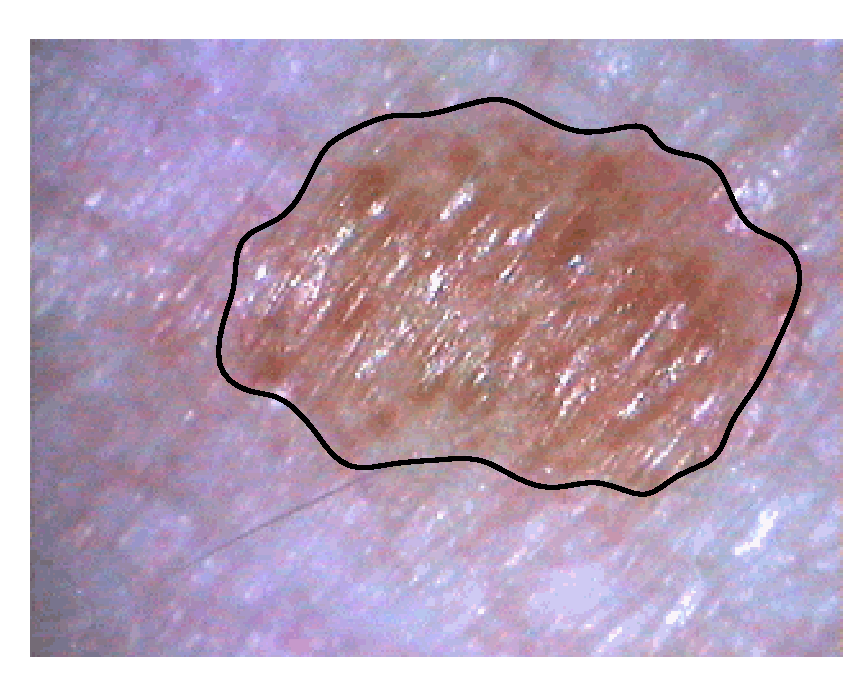
\psfig{file="./images/ris1I1.eps",height=5cm,clip=}}
 \centerline{
  \psfig{file="./images/rI2o.eps",height=5cm,clip=}
   \hfill
  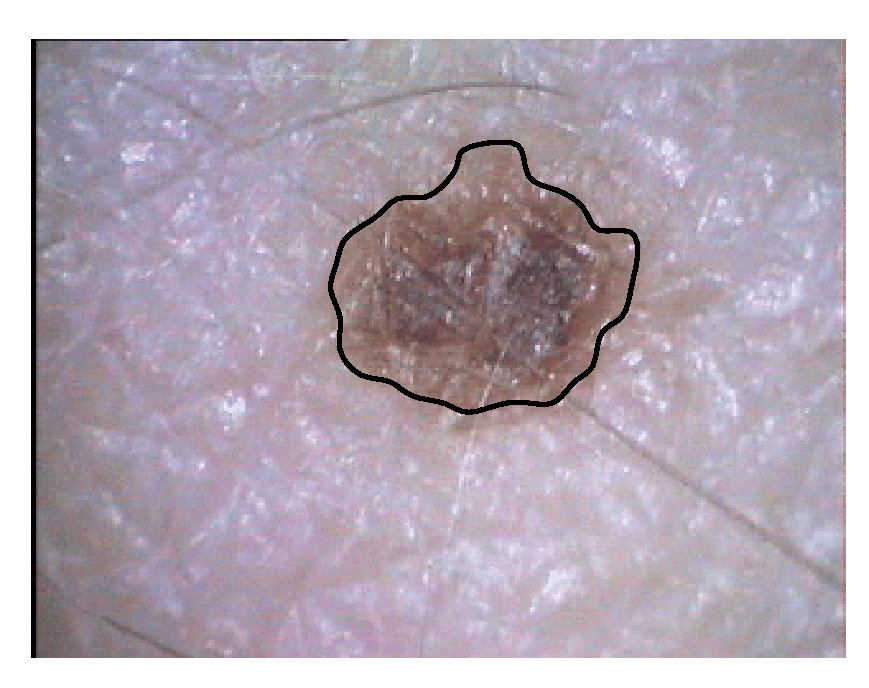
\psfig{file="./images/rI2f.eps",height=5cm,clip=}}
   \caption[Risultato della segmentazione con inizializzazione manuale]
    {{\sl A sinistra}: inizializzazione manuale del contorno iniziale; sono evidenziati i $4$
     punti di controllo e la curva a B-splines che li approssima. {\sl A destra}: risultato 
     della segmentazione.}
 \lb{risIm}
\end{figure}

\begin{figure}[tbp]
 \centerline{
  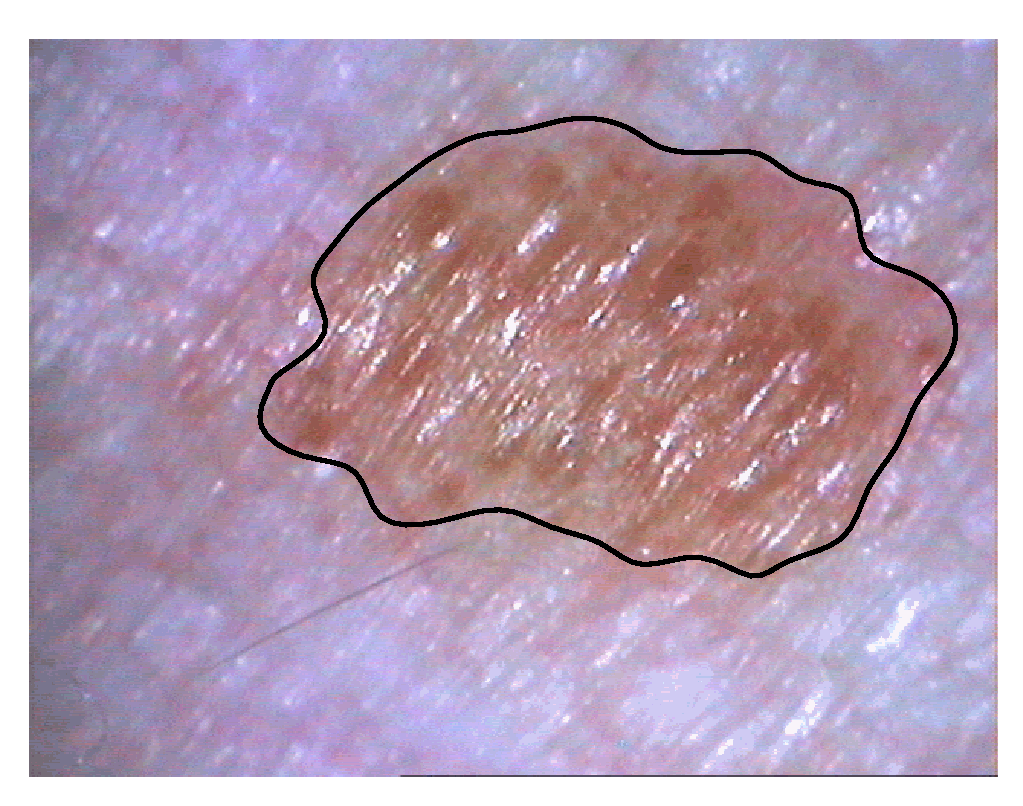
\psfig{file="./images/segfin1.eps",height=5cm,clip=}
   \hfill
  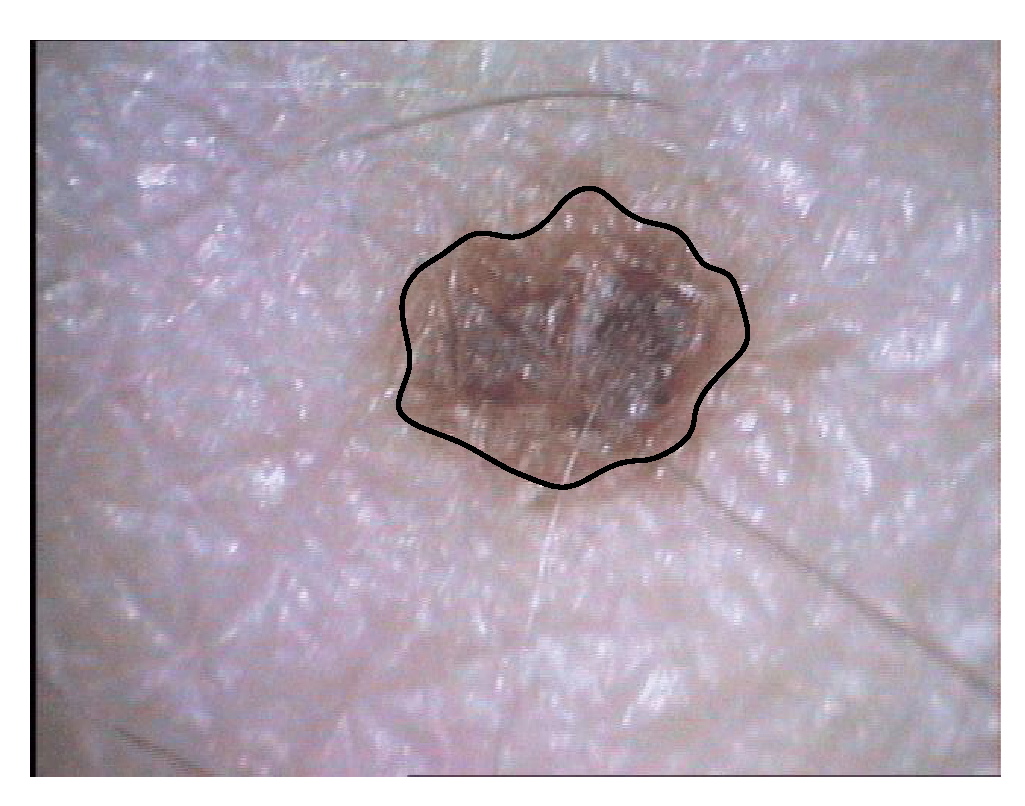
\psfig{file="./images/segfin2.eps",height=5cm,clip=}}
   \caption[Risultato della segmentazione con inizializzazione semiautomatica]
    {Due risultati dell'applicazione dell'algoritmo di segmentazione con inizializzazione
     semiautomatica, dove il contorno iniziale \e ricavato dal bordo della regione compatta
     ottenuta dalla binarizzazione della componenete principale della trasformata di K.L.
     dell'immagine originale.}
 \lb{risIsa}
\end{figure}

\begin{figure}[tbp]
 \centerline{
  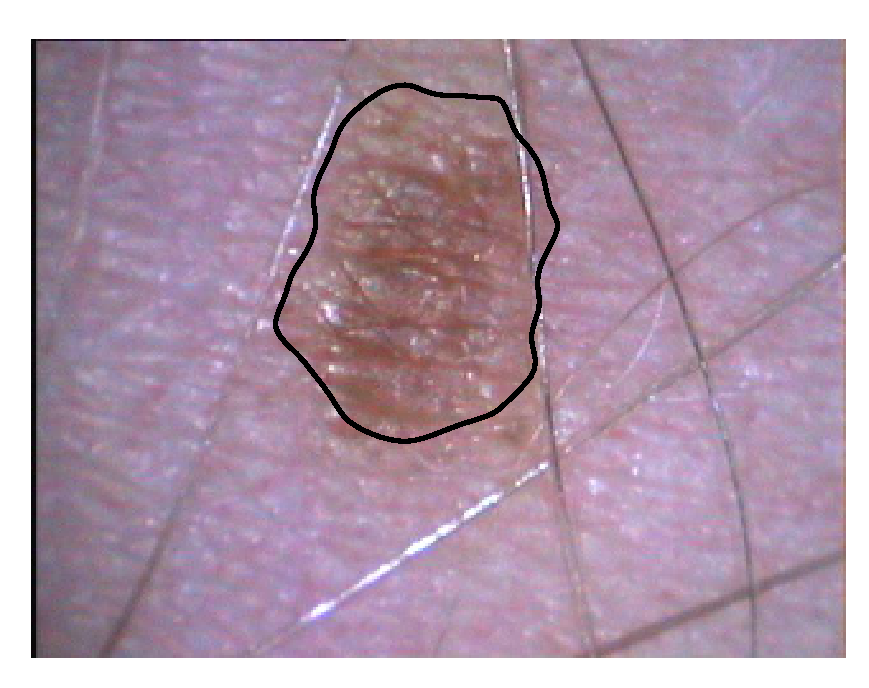
\psfig{file="./images/r3I9.eps",height=5cm,clip=}
   \hfill
  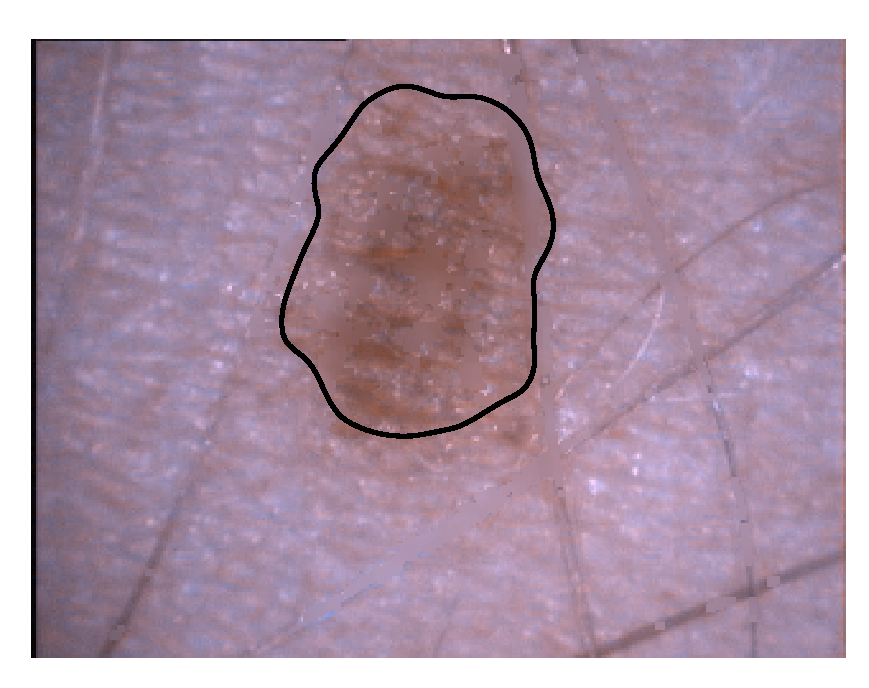
\psfig{file="./images/r2I9.eps",height=5cm,clip=}}
   \caption[Risultato della segmentazione con l'applicazione di un operatore anisotropo per la
    riduzione dei disturbi]
    {{\sl A sinistra}: applicazione dell'algoritmo di segmentazione direttamente all'immagine
     originale. {\sl A destra}: il processo di segmentazione \e preceduto da una fase di 
     preelaborazione in cui si riduce l'effetto di disturbo dei peli con l'applicazione
     di un operatore locale anisotropo.}
 \lb{risIp}
\end{figure}

 

